%--------------------------------------------
%	PACKAGES AND DOCUMENT CONFIGURATIONS
%--------------------------------------------

\documentclass[11pt]{article}
\usepackage{fancyhdr}
\usepackage{pgfplots}
\usepackage{gensymb}
\usepackage[ampersand]{easylist}
\usepackage[a4paper, total={8.5in, 11in}, margin = 1in]{geometry}

\usepackage[version=3]{mhchem} % Package for chemical equations
\usepackage{siunitx} % The \SI{}{} and \si{} command for SI units
\usepackage{graphicx, epstopdf} % Required for the inclusion of images
\usepackage{natbib} % Required to change bibliography style to APA
\usepackage{amsmath} % Required for some math elements
\usepackage[framed,numbered]{matlab-prettifier}
\usepackage{float}
\usepackage{multirow}
\usepackage{listings}
\usepackage{setspace}
\doublespacing

\setlength\parindent{2em} % Removes all indentation from paragraphs

\renewcommand{\labelenumi}{\alph{enumi}.} % Make numbering in the enumerate environment by letter rather than number 

\setcitestyle{square}

%----------------------------------------------
%	DOCUMENT INFORMATION
%----------------------------------------------
\title{\Bathsoap Extract and Pharmaceutical Cases\\ \vspace{1.0cm}
Assignment 2 \\
\\ \vspace{1.0cm}
Name: Whitney Chu\\
}

   
\date{Date: Wednesday, December 16th, 2020}

\newpage

\begin{document}

\begin{titlepage}
    \centering
    \maketitle
    \thispagestyle{empty}
\end{titlepage}

\pagebreak


\newpage
\thispagestyle{empty}
\tableofcontents
\newpage


\newpage
\pagenumbering{arabic}



\section{Bathsoap Extracts Case}
There are multiple different variables that can be used to describe brand loyalty according to the three different measures. The variables that can potentially describe brand loyalty are number of brands purchased, average number of transactions and average transaction per brand which is calculated by dividing the number of transactions by the number of brands.

The brand loyalty measures are all different in the sense that they are a different sort of measurement. Visualizations of all three brand loyalty measures can be seen in the appendix. Before creating the visualizations, I created a field called “row count” that counts the number of rows, as each household represents a household. This calculated field made it easier to compare the number of households that buy different number of brands. Brand loyalty measure 1 compares the number of households against the number of brands purchased. From the visualization, it can be seen that majority of households typically buy 3 different brands and it is rare that household buy from 9 different brands. It is also evident that not many households are loyal to one brand only, and theoretically this makes sense, because not many people only buy one specific brand. This may be due to many factors, for example if another brand has a promotion or sale, people may want to buy the product they want with the cheaper price, even if it is a different brand.  Brand loyalty measure 2 displays the number of brands purchased against the average transaction per brand. There are multiple different ways to display this loyalty measures, so I chose three different visualizations to display the information. From the first visualization it can be seen that the highest average transaction per brand is when the customer purchases 9 different brands and the lowest average transaction per brand is when the customer purchases 6 different brands. There may be high transaction per brand for the customers that purchase 9 brands, however the number above the bar on the graph shows that only 2 households buy 9 different brands. The second visualizations shows the average transaction per brand and you can see that many customers buy from a brand on average 8 times. The third visualization displays the number of runs purchasing the same brand and you can see that many households have 17 runs. This is not a good loyalty measure, because If someone is loyal only to one brand, they may take up all the transactions and that is not a good representation of the households that brands should target. It can also be seen that although only 37 household are loyal to only one specific brand, they have a decently high average transaction per brand value. This is very different than brand loyalty measure 1 because it displays the average transaction per brand without considering the number of households in each category. Brand loyalty measure 3 compares the number of brands purchased with the average number of transactions. I used two different visualizations to display this loyalty measure. From this visualization, it can be established that the average number of transactions is highest when 9 different brands are purchased and the average number of transactions is the lowest when only 1 brand is purchased. The order of transactions goes is descending order from 9 to 1. This is a very evident result as the more brands bought, the higher the overall number of transactions. This is not a good representation of brand loyalty because it is categorizing transactions as a whole and not per brand, so it is obvious that the number of transactions for only one brand is going to be the lowest. This does not represent the amount of households that buy specific brands and therefore doe not represent how loyal a customer is to a specific brand. The second visualization looks at specific brands and the customers according to socio economic class. From this, it is evident that the socio economic class 4 has not spent a lot of money on all the brands and tends to spend more money on certain brands. This means that those of higher socio economic class have more brand loyalty towards specific brands. 

Brand loyalty measure 3 should be used for targeting promotions because it tells the information about the overall transactions by household for each brand. Therefore, the brand will know which household to target.  For example, brand loyalty 3 tells you that they should target loyal customers to that brand, but you can also target those who are loyal to multiple brands. Brand loyalty measure 1 and 2 present information that is not useful for determining which households to target when they want to have a sale or promotion. Brand loyalty measure 3 makes it easy to display whether a promotion is working because then the number of transactions will increase and there will be more households that buy more brands. For those that only buy one brand and now they go for the promotion, they will now go into the category of 2 brands. For those that buy 4 brands and go for the promotion will now go into the category of 5 brands. This is how we can tell how effective a promotion is.  

	
The percentage of total purchases comprised by various brands shows the number of households that purchase more than one brand. Brands should use this information to target specific households in order to increase their total purchases. Using sales and promotions is a good way for brands to attract more customers. 
	
A customer who buys all brand A is not necessarily just as loyal as a customer who only buys brand B. Over time, or in certain situations, the customer may not be as loyal as they seem to be. For example, if there is a good promotion on a product but it is a different brand, the customer may buy that brand instead meaning they are not as loyal. Customers may only be loyal for a certain time period and then may not be loyal later on. 

The average price of products bought is higher with less number of brands purchased. This  means that customers with more loyalty pay a higher average price. This could be due to the fact that if people are more loyal they won’t choose other brands even if other brands have promotions and will pay a higher price for the same brand, therefore increasing the average price. The visualization for this relationship can be seen in the appendix. It can be seen that the lowest average price is associated with 9 brands purchased meaning they do not have brand loyalty.	

When there are more brands purchased, there is a lower average volume per transaction. When you buy more brands there will be less volume of each product you buy, as the products you buy are split between different brands. Therefore when there is less volume per transaction, this means there is less brand loyalty. The visualization for this relationship can be seen in the appendix. It is evident that the lowest average volume per transaction is associated with 9 brands purchased. 

For promotions, Brands should target customers that purchase multiple different brands. These customers tend to be open to buying multiple different brands and may be more enticed if there is a promotion. I created visualizations to compare socio economic class, age, number of children, household size, food eating habits and television to the number of brands purchased by customers. These visualizations can be seen in the appendix. It is evident that higher socio economic class is typically associated with more brand loyalty in the sense that they stick to only one brand and don’t switch between brands. These customers tend to have more money and may not consider promotions and just buy the brands they like, so these are not good customers to target. Brands should segment their promotions to customers that are of lower socio economic class but they can also target customers that they know are only loyal to them. From the visualization it can be seen that older aged people have more brand loyalty towards one brand because they are more established and can afford the brands they want, meaning they may not go for promotions. Brands should target younger aged people as they typically have less money and look for promotions for reduced prices. It can also be seen that customers that have more kids and larger household size are less likely to be loyal to one brand and typically buy from multiple brands and will most likely go for promotions. With more kids, expenses are higher and in order to save money, families look for promotions and discounts on products they need and want, so brands should target larger families. Brands should also target non-vegetarians because vegetarians are typically loyal to one brand as there are limited brands that offer vegetarian options. Customers that have television are more likely to up to date with the products available and the promotions going on, so brands should target customers that have television to get the word across faster and effectively. Customers will see commercials with promoted products and if they like it, they will buy it, which will increase overall volume of transactions. Theoretically, If a brand knows for sure a customer is loyal, they can target them and if a brand sees that a customer is loyal to multiple brands, they should target them as well. Those who are loyal to multiple brands are more likely to not be set on only buying one brand and if they see a promotion, they may be open to switching brands. 

\section{Pharmaceuticals Case}
The first step was adding all the variables into the clusters in order to determine which ones were significant. I looked at all the variables with a p-value of less than 0.05 and removed the ones that were over 0.05. The variables chosen were market capitalization, net profit margin, asset turnover, revenue growth and ROA. The variables that were not significant that had a p-value over 0.05 were beta, leverage, ROE and PE ratio. The p-value of the variables can be seen in the appendix. The number of clusters was not chosen by me, as it was mentioned in class that it is best to leave the clusters as “automatic” on tableau to get the optimal number of clusters. The optimal number of clusters turned out to be 4 and a scatterplot of the clusters can be seen in the appendix.

Before analyzing the clusters, I looked at the meaning of each significant variable. Market capitalization gives an overview of the company’s worth and how it compares to other companies. Return on assets indicates how profitable a company is based on its assets. Asset turnover measures the value of a company’s sales divided by its assets. Estimated revenue growth is essentially an estimate of the future worth of the company’s stock by comparing growth between periods. Net profit margin determines the amount of income acquired as a percentage of revenue. With respect to all these variables, the larger the values, the better. From analyzing the details of the clusters, it can be seen that cluster 2 includes the companies that have the best value, have performed well and have a high estimated revenue growth. All the variables in cluster 2 have high values. All the variable in cluster 1 also have decently high values, but not as high as cluster 2.  This means cluster 1 is valued well and has a decently good performance overall. Cluster 3 has a high market cap and asset turnover, whereas Cluster 4 has a high net profit margin, revenue growth and ROA. Cluster 4 has more high values than cluster 3 indicating it has a better performance. Cluster 3 therefore has the worst performance out of all the clusters based on the financial variables. 
	
The three categorical variables were not used in forming the clusters, however a new scatterplot with the previous details was formed and displayed the details of these categorical variables. When looking at the categorical variables compared to the clusters, different patterns and trends can be seen. The most significant variable within the clusters is the ROA, so this variable was used as the inputs when comparing the categorical variable to the clusters. Tables visualizations of the median recommendation, location and exchange in the clusters can be seen in the appendix. From the table of median recommendation in the clusters, it can be seen that the “strong buy” category is only in cluster 3, “moderate sell” category is only in cluster 1 and 4, “hold” category is in cluster 1,2 and 3, and the category “moderate buy” is in all four clusters. From the table of location in the clusters, it can be seen that Canada is only in cluster 3, France is only in cluster 4, Germany is only in cluster 3, Ireland is only in cluster 4, Switzerland is only in cluster 1, UK is in cluster 1,2 and 3 and US is in all four clusters. From the exchange in cluster table, it can be seen that AMEX and NASDAQ are only in cluster 3 and NYSE is seen in all four clusters. 

When looking at the names of each data point in the clusters, it can be seen that cluster 2 contains the large, well-known pharmaceutical companies like Johnson-and-Johnson. It is also evident that the market cap and net profit margin are both high values for cluster 2. With this information and the financial information, an appropriate name for this cluster would be “well-known, successful pharmaceutical companies”. Cluster 1 has medium values for market cap and high values for net profit margin. Therefore an appropriate name for cluster 1 would be “profitable, well-valued pharmaceutical companies”. Cluster 4 contains points with only NYSE and moderate sell/buy with medium values for net profit margin and low market cap. Therefore, an appropriate name for cluster 4 would be “Companies with moderate sell and buy”. Cluster 3 contains a strong buy, moderate buy and hold as median recommendation, low values for market cap and low values for net profit margin. Therefore, an appropriate name for cluster 3 would be “less profitable, strong hold companies”.


\newpage
\pagenumbering{arabic}% resets `page` counter to 1
\renewcommand*{\thepage}{A\arabic{page}}
\appendix 

\section{Appendix}
\subsection{Bathsoap Extracts Case}
\subsubsection{Brand Loyalty Measure 1}
\begin{figure}[H]
    \centering
    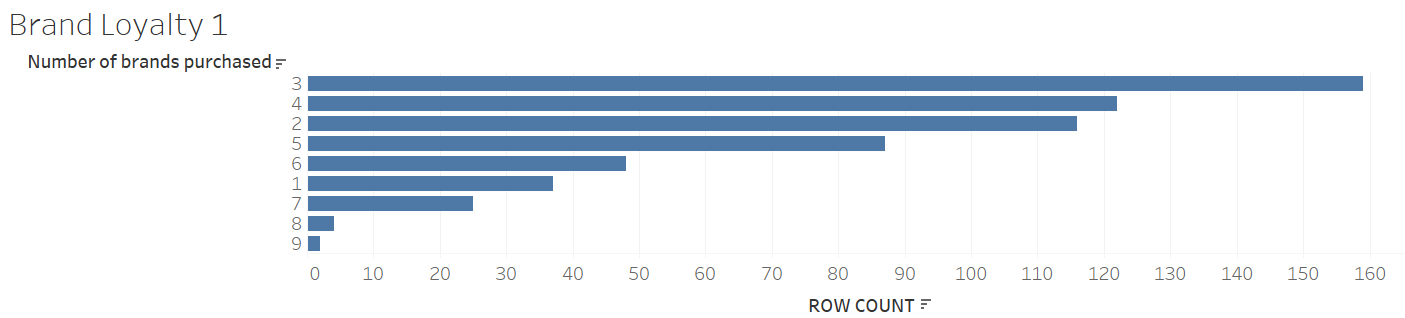
\includegraphics[width=1\columnwidth]{pics/bl1.png}
    \caption{Brand Loyalty Measure 1}
    \label{lr}
\end{figure}

\subsubsection{Brand Loyalty Measure 2}
\begin{figure}[H]
    \centering
    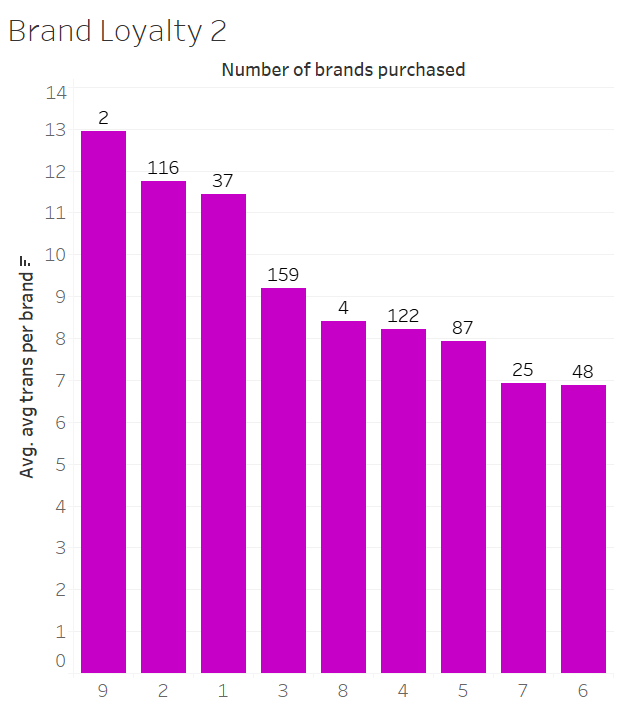
\includegraphics[width=0.65\columnwidth]{pics/bl2.png}
    \caption{Brand Loyalty Measure 2 Visualization 1}
    \label{lr}
\end{figure}

\begin{figure}[H]
    \centering
    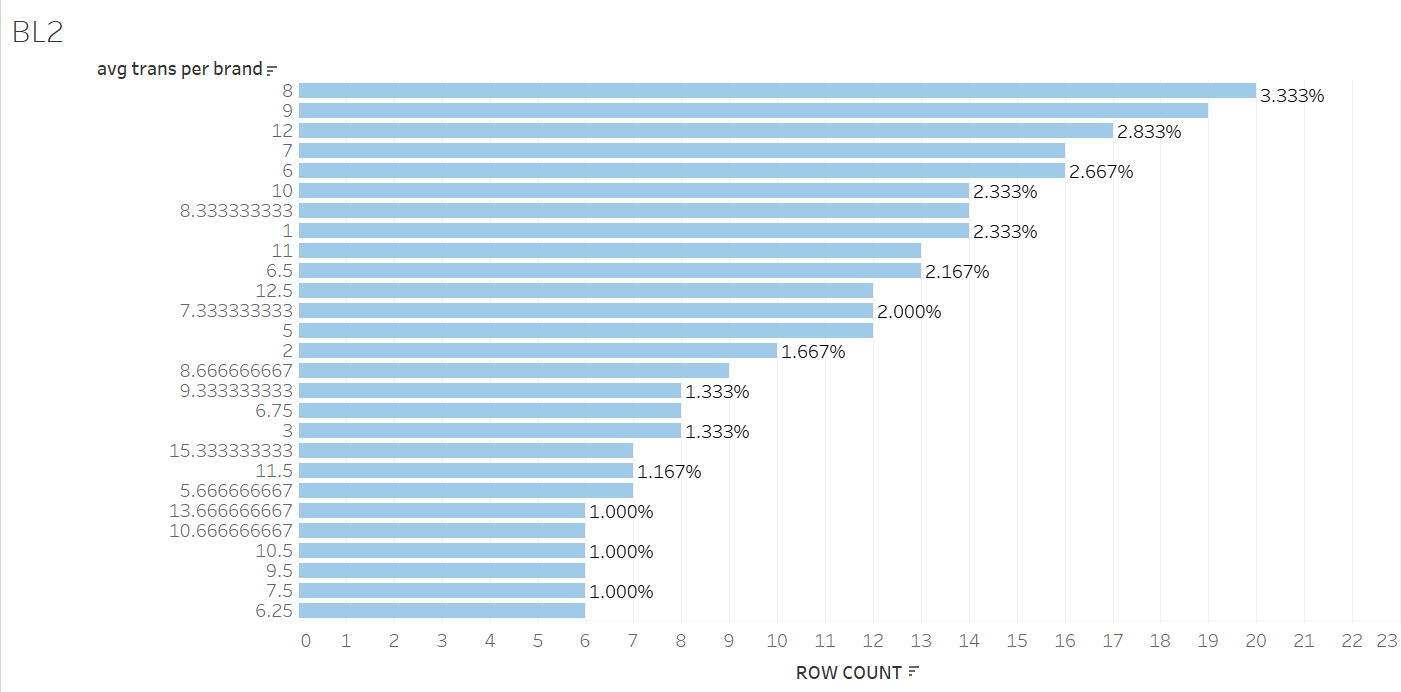
\includegraphics[width=0.9\columnwidth]{bl22.png}
    \caption{Brand Loyalty Measure 2 Visualization 2}
    \label{lr}
\end{figure}

\begin{figure}[H]
    \centering
    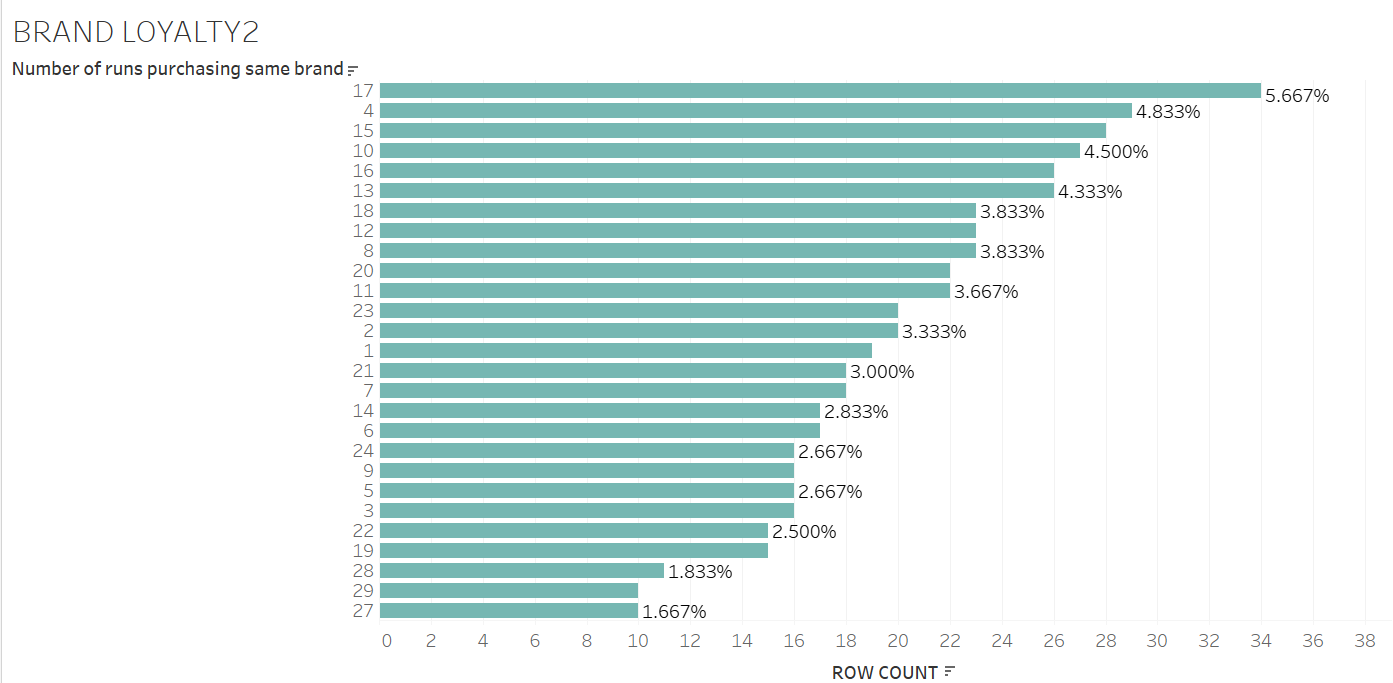
\includegraphics[width=0.9\columnwidth]{bl222.png}
    \caption{Brand Loyalty Measure 2 Visualization 3 }
    \label{lr}
\end{figure}

\subsubsection{Brand Loyalty Measure 3}
\begin{figure}[H]
    \centering
    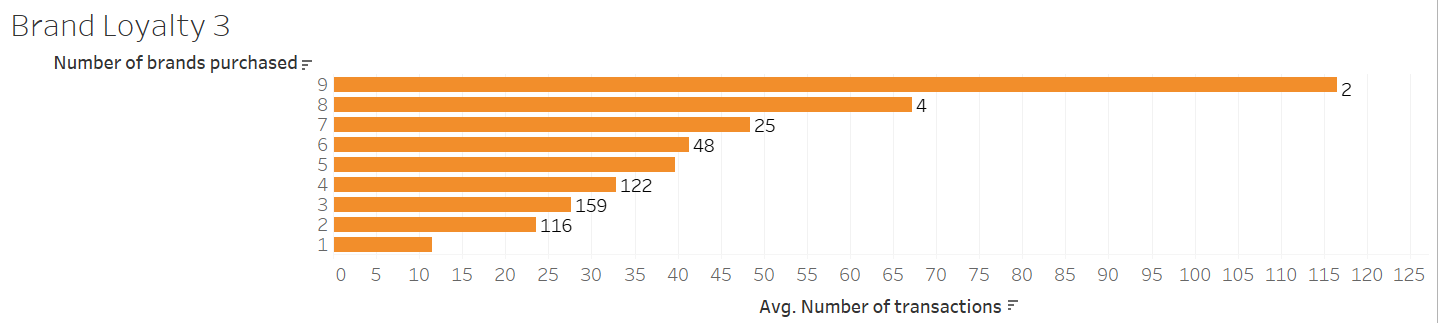
\includegraphics[width=1\columnwidth]{pics/bl3.png}
    \caption{Brand Loyalty Measure 3 Visualizatoin 1}
    \label{lr}
\end{figure}

\begin{figure}[H]
    \centering
    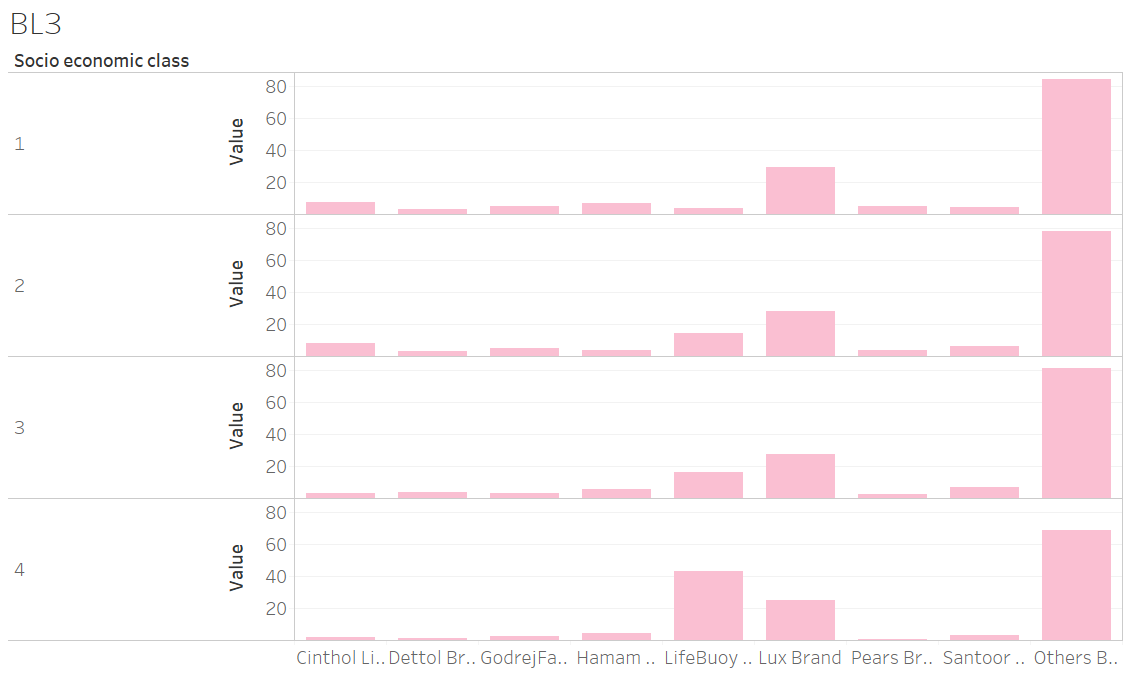
\includegraphics[width=1\columnwidth]{bl33.png}
    \caption{Brand Loyalty Measure 3 Visualization 2}
    \label{lr}
\end{figure}

\subsubsection{Average Price vs Number of Brands}
\begin{figure}[H]
    \centering
    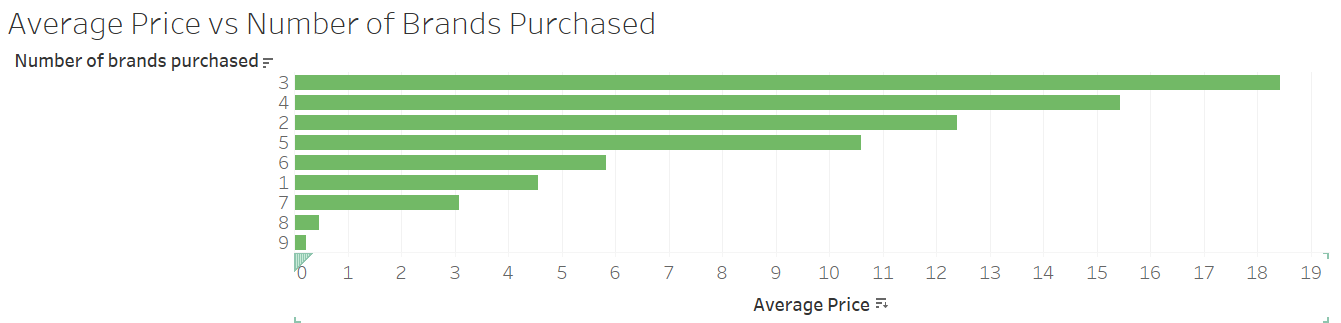
\includegraphics[width=0.9\columnwidth]{price.png}
    \caption{Average Price vs Number of Brands}
    \label{lr}
\end{figure}

\subsubsection{Average Volume vs Number of Brands}
\begin{figure}[H]
    \centering
    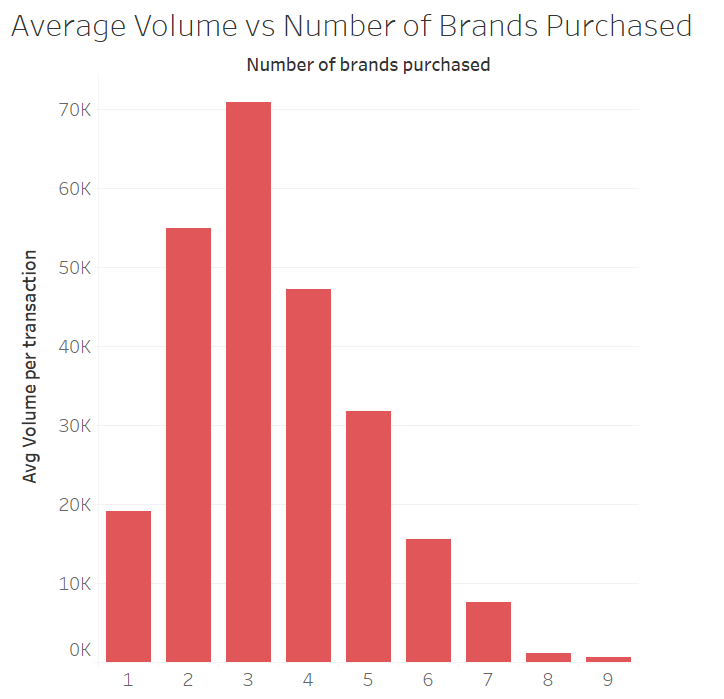
\includegraphics[width=1\columnwidth]{volume.png}
    \caption{Average Volume vs Number of Brands}
    \label{lr}
\end{figure}

\subsubsection{Socio Economic Class vs Number of Brands}
\begin{figure}[H]
    \centering
    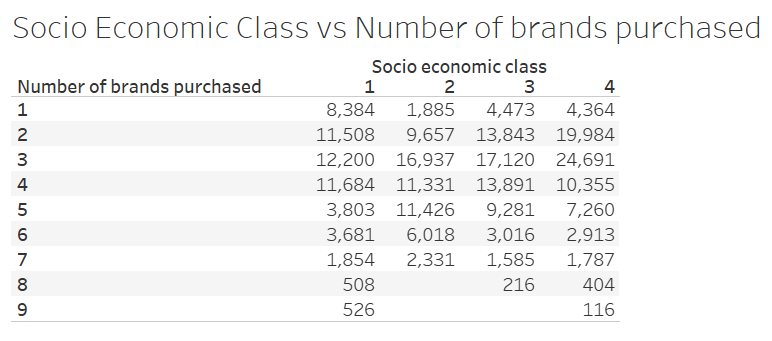
\includegraphics[width=1\columnwidth]{sec.png}
    \caption{Socio Economic Class vs Number of Brands}
    \label{lr}
\end{figure}

\subsubsection{Age vs Number of Brands}
\begin{figure}[H]
    \centering
    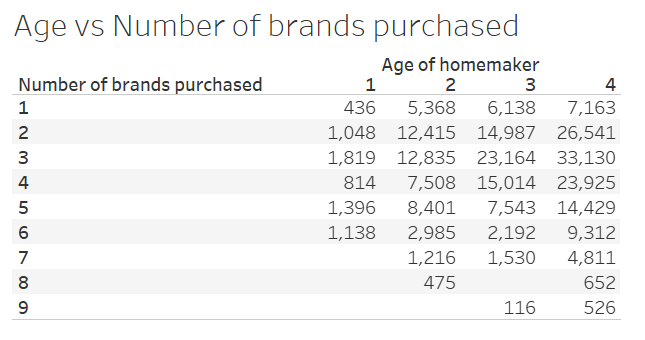
\includegraphics[width=1\columnwidth]{age.png}
    \caption{Age vs Number of Brands}
    \label{lr}
\end{figure}

\subsubsection{Child vs Number of Brands}
\begin{figure}[H]
    \centering
    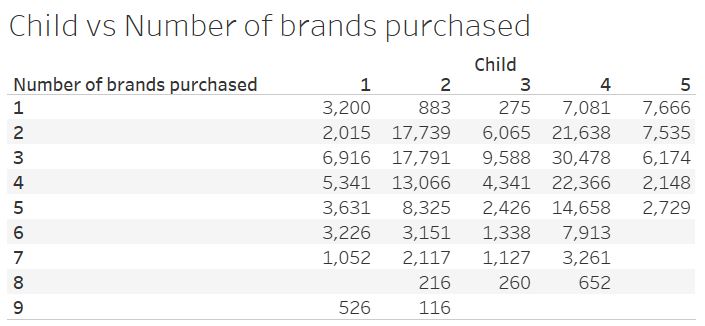
\includegraphics[width=1\columnwidth]{child.png}
    \caption{Child vs Number of Brands}
    \label{lr}
\end{figure}

\subsubsection{Household Size vs Number of Brands}
\begin{figure}[H]
    \centering
    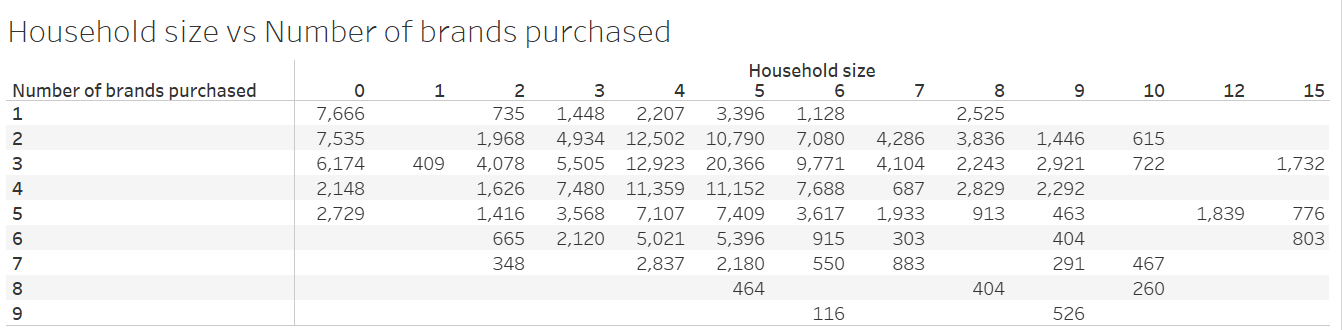
\includegraphics[width=1\columnwidth]{hh.png}
    \caption{Household Size vs Number of Brands}
    \label{lr}
\end{figure}

\subsubsection{Food Eating Habits vs Number of Brands}
\begin{figure}[H]
    \centering
    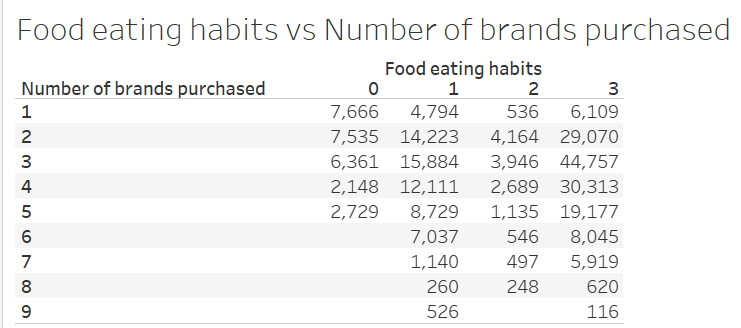
\includegraphics[width=1\columnwidth]{food.png}
    \caption{Food Eating Habits vs Number of Brands}
    \label{lr}
\end{figure}

\subsubsection{Television vs Number of Brands}
\begin{figure}[H]
    \centering
    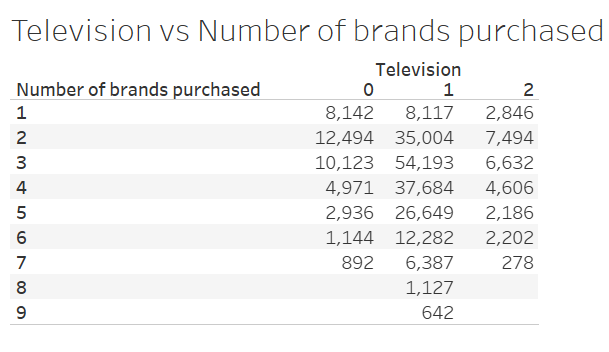
\includegraphics[width=1\columnwidth]{tv.png}
    \caption{Television vs Number of Brands}
    \label{lr}
\end{figure}

\newpage




\subsection{Pharmaceuticals Case}
\subsubsection{P-values of Variables}
\begin{figure}[H]
    \centering
    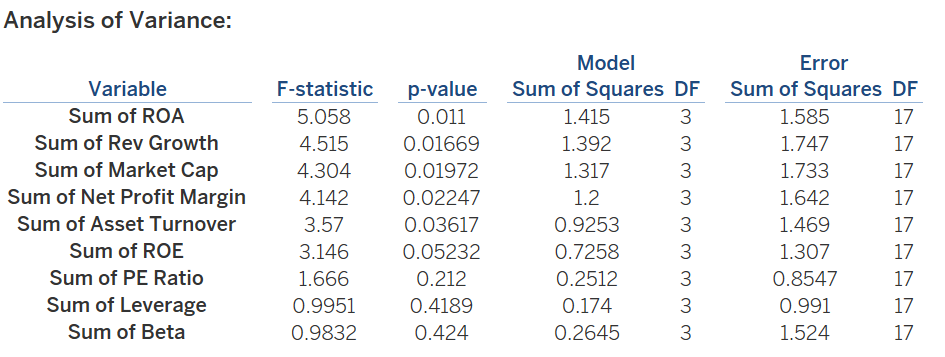
\includegraphics[width=0.90\columnwidth]{pics/pv.png}
    \caption{P-values of Variables}
    \label{lr}
\end{figure}

\subsubsection{Scatterplot of Clusters with significant variables}
\begin{figure}[H]
    \centering
    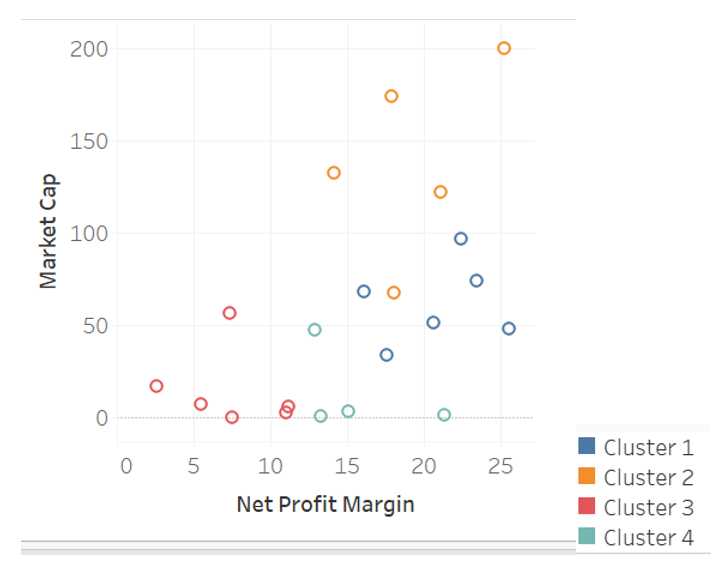
\includegraphics[width=0.92\columnwidth]{pics/clust.png}
    \caption{Scatterplot oc Clusters with significant variables}
    \label{lr}
\end{figure}

\subsubsection{Description of Clusters}
\begin{figure}[H]
    \centering
    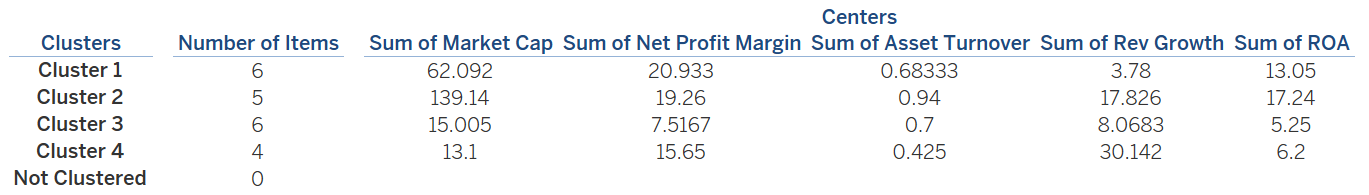
\includegraphics[width=0.98\columnwidth]{pics/desc.PNG}
    \caption{Description of Clusters }
    \label{lr}
\end{figure}

\subsubsection{Median Recommendation in Clusters}
\begin{figure}[H]
    \centering
    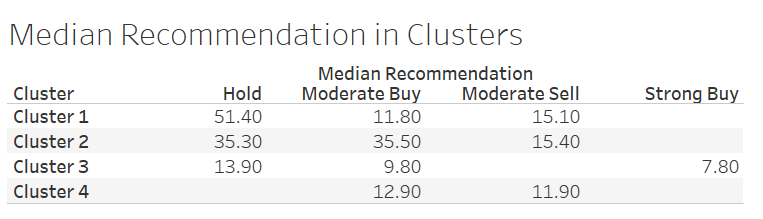
\includegraphics[width=0.90\columnwidth]{pics/mr.png}
    \caption{Median Recommendation in Clusters}
    \label{lr}
\end{figure}

\subsubsection{Location in Clusters}
\begin{figure}[H]
    \centering
    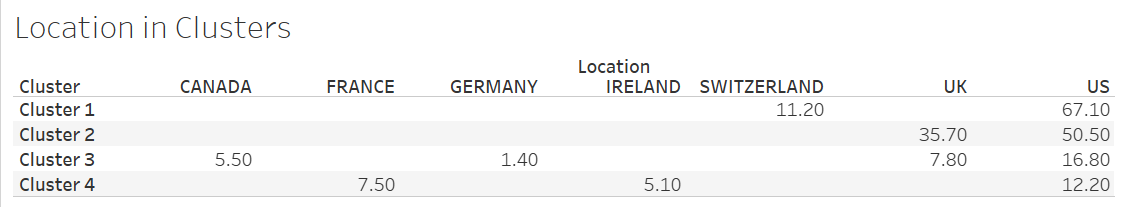
\includegraphics[width=0.98\columnwidth]{pics/loc.png}
    \caption{Location in Clusters}
    \label{lr}
\end{figure}

\subsubsection{Exchange in Clusters}
\begin{figure}[H]
    \centering
    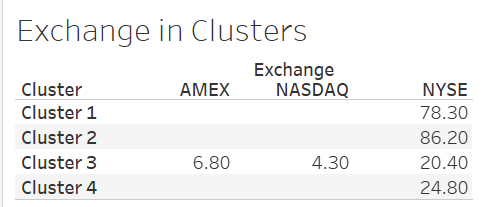
\includegraphics[width=0.90\columnwidth]{pics/exch.png}
    \caption{Exchange in Clusters}
    \label{lr}
\end{figure}



\end{document}